\documentclass[12pt,a4paper]{article}
\usepackage{physics}
\usepackage{amssymb}
\usepackage{subcaption}
\usepackage{colortbl}
\newcommand{\activity}{Activity 6 -- Enhancing Color Images}
\input{spp.dat}

%  Editorial staff will uncomment the next line
% \providecommand{\artnum}[0]{XX-XX}
% \renewcommand{\articlenum}[0]{SPP-\the\year-\artnum-}

\begin{document}

\title{\TitleFont \activity}
\author[ ]{\textbf{Kenneth V. Domingo} \\
2015--03116 \\
App Physics 186, 1\textsuperscript{st} Semester, A.Y. 2019--20}
\affil[ ]{\corremail{kvdomingo@up.edu.ph} }

\maketitle
\thispagestyle{titlestyle}

\section*{Results and Discussion}
\setcounter{section}{1}

For this activity, I will be using the raw image (Fig. \ref{fig:orig}) I took during the FST Week Concert at the College of Fine Arts. I felt this would be a good image to work on since there is a significant and discernible color cast due to the lighting of the venue. The photo was taken with auto white balance (which didn't do a really good job of white balancing).

\subsection{Contrast stretching}
I imported the original image as \texttt{uint8}. However, when performing any manipulation, I converted it first to \texttt{float64} before casting it back to \texttt{uint8} for displaying and saving purposes. Upon examination, I realized it was futile to perform contrast stretching since the maximum value of each channel was already 1.0. Further reading brought me to an article \cite{constretch}, where we can discard a certain percentile from the low and high ends of the histogram and stretch the remaining bins to fill the full range, according to

\begin{equation}\label{eq:constretch}
	I_C^\prime = \frac{I_C - C_{low}}{C_{high} - C_{low}} \times C_{\max} + C_{\min}
\end{equation}

\noindent
where $C$ refers to the channel being manipulated. The \textit{high} and \textit{low} values refer to the $p$th percentile of histogram values that are set as the upper and lower thresholds, respectively. This is actually the algorithm used by GIMP's auto white balance. We can see from the resulting image in Fig. \ref{fig:constretch} that the reddish color cast has generally been removed, and the guitarist's skin tone looks much more realistic.

\subsection{Gray world}
This algorithm assumes that the average color of the image is gray. The pixel values are manipulated according to \cite{soriano}

\begin{equation}\label{eq:grayworld}
	I_C^\prime = I_C \times \frac{\ev{I}}{\ev{C}}
\end{equation}

\noindent
where $\ev{I}$ is the overall average and $\ev{C}$ is the channel average. The result of this manipulation is shown in Fig. \ref{fig:grayworld}. Note that the image is at roughly the same exposure level as the original because we did not perform contrast stretching on this one, but the white balance is similar to that of contrast stretching.

\subsection{White patch}
This method is similar to how the White Balance Eyedropper Tool in image processing programs such as Lightroom or Photoshop work. Fig. \ref{fig:patch} shows the location where I extracted a patch that is supposed to be white (upper 12th fret marker on the guitar). The result is shown in Fig. \ref{fig:whitepatch}. We can see that the guitarist's skin tone still looks realistic, and the background is now a warmer white as compared to the previous algorithms.

\begin{figure}[htb]
	\centering
	\begin{subfigure}[h!]{0.24\textwidth}
		\centering
		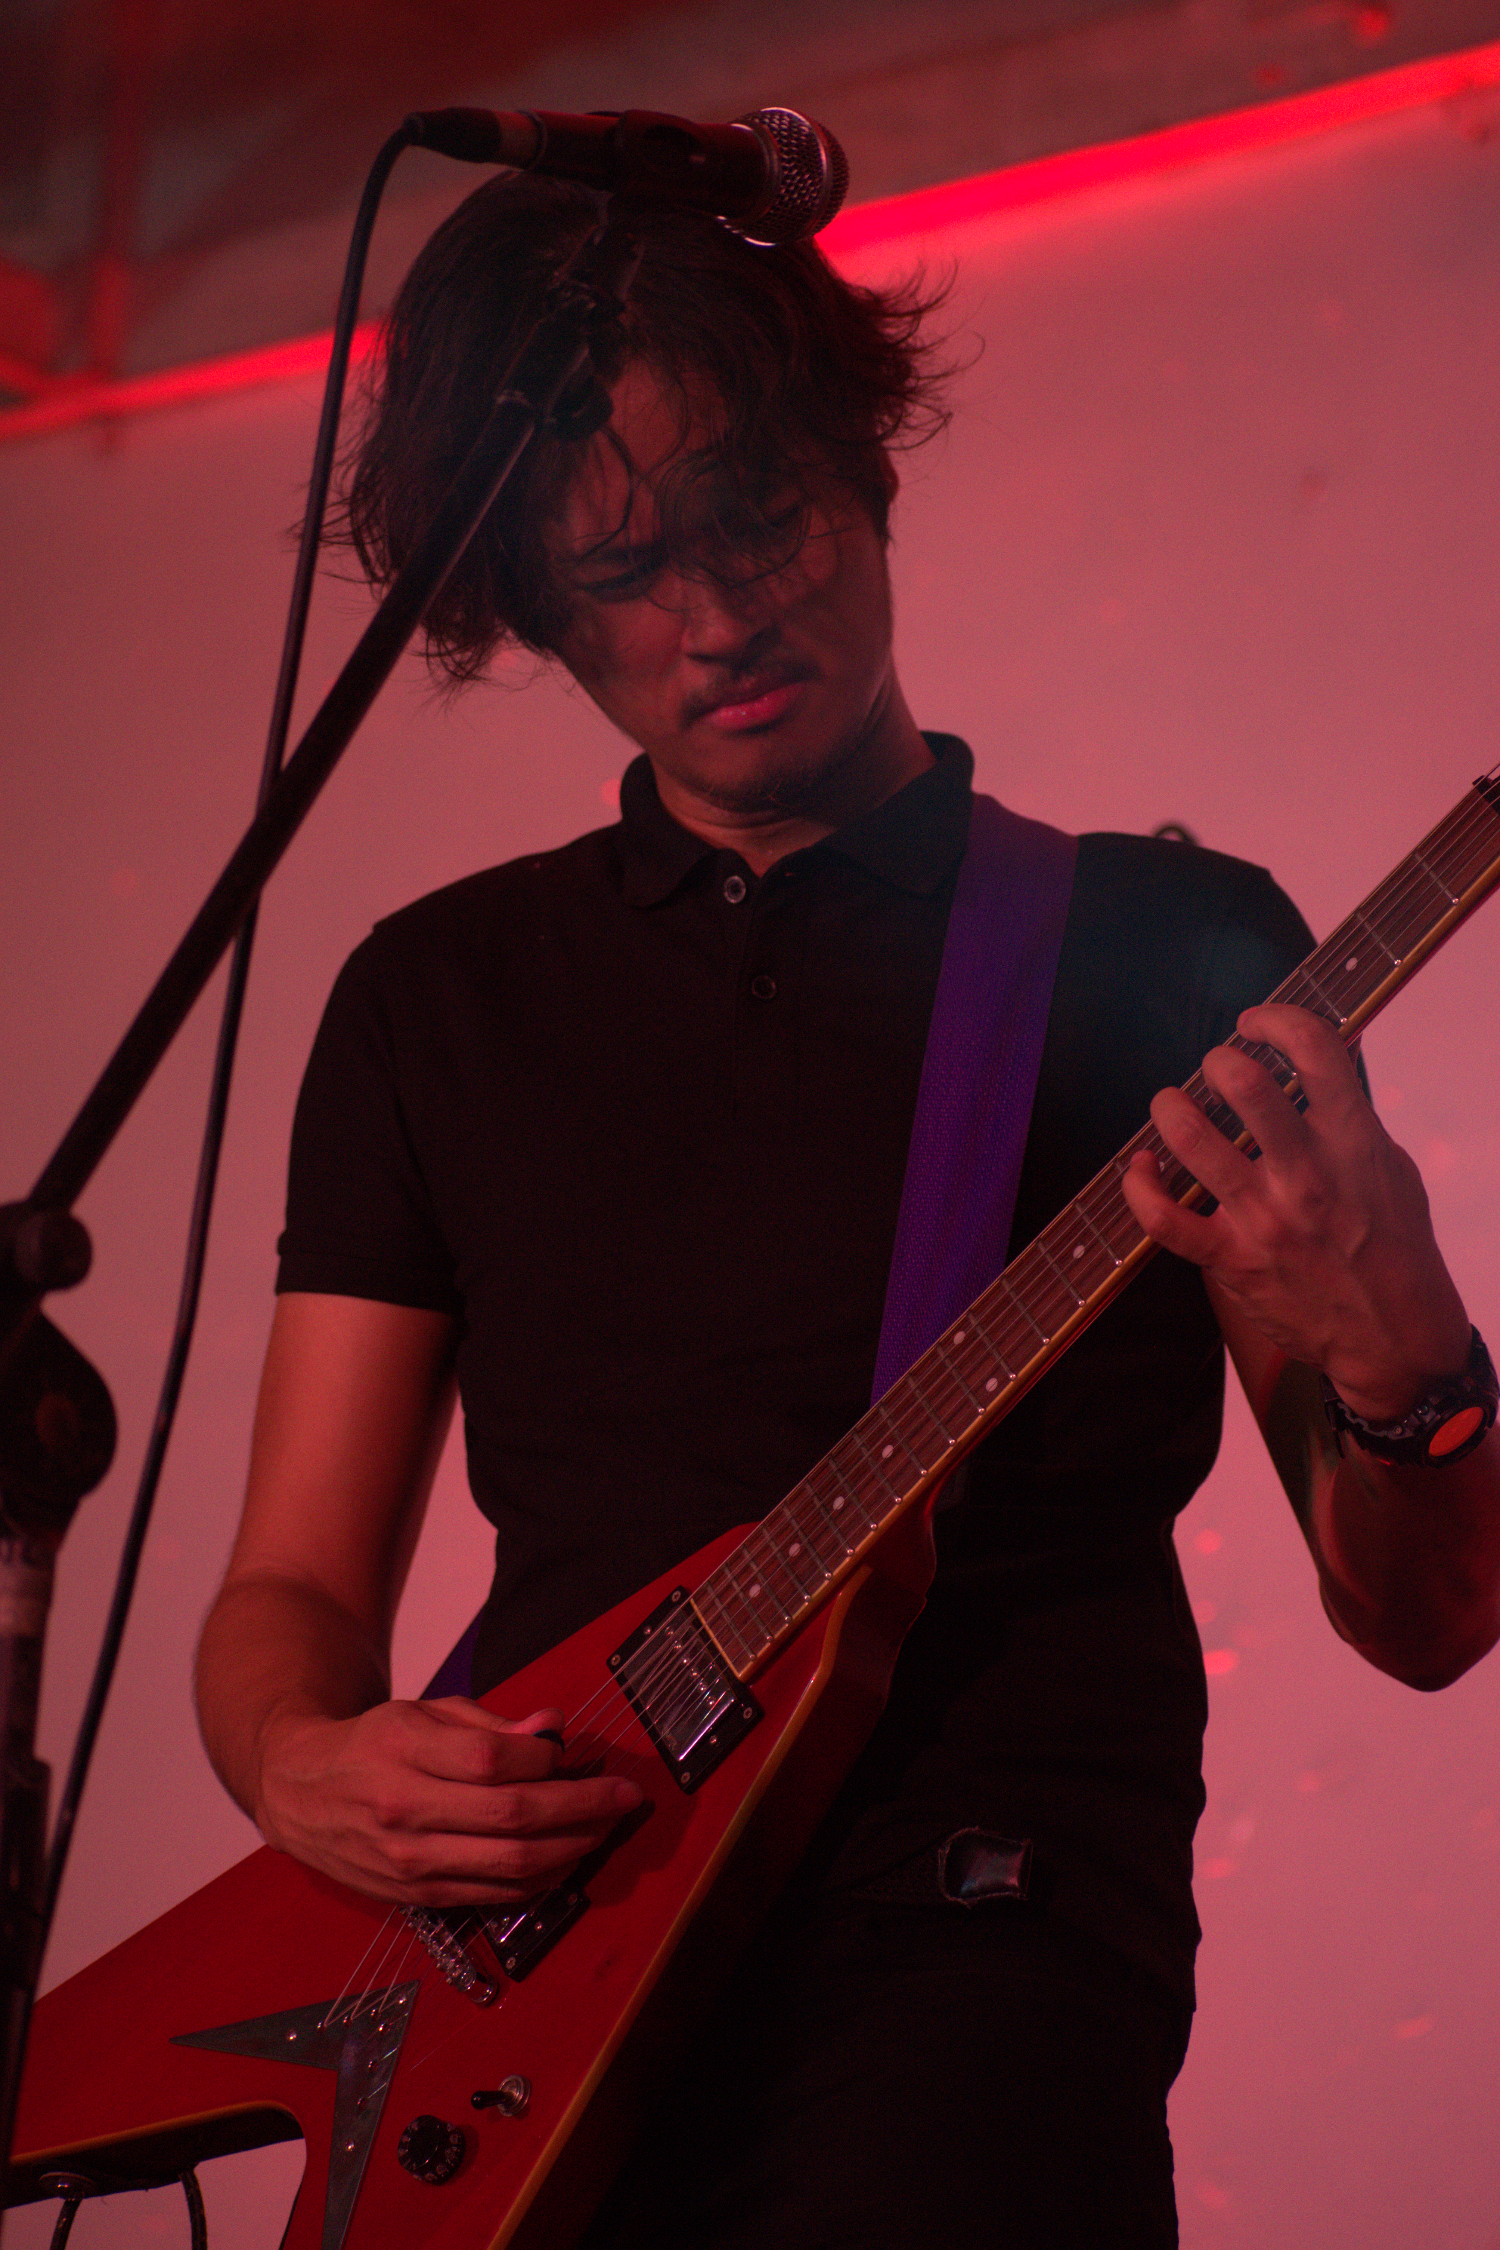
\includegraphics[width=\textwidth]{original.png}
		\caption{Original image}
		\label{fig:orig}
	\end{subfigure}
	\begin{subfigure}[h!]{0.24\textwidth}
		\centering
		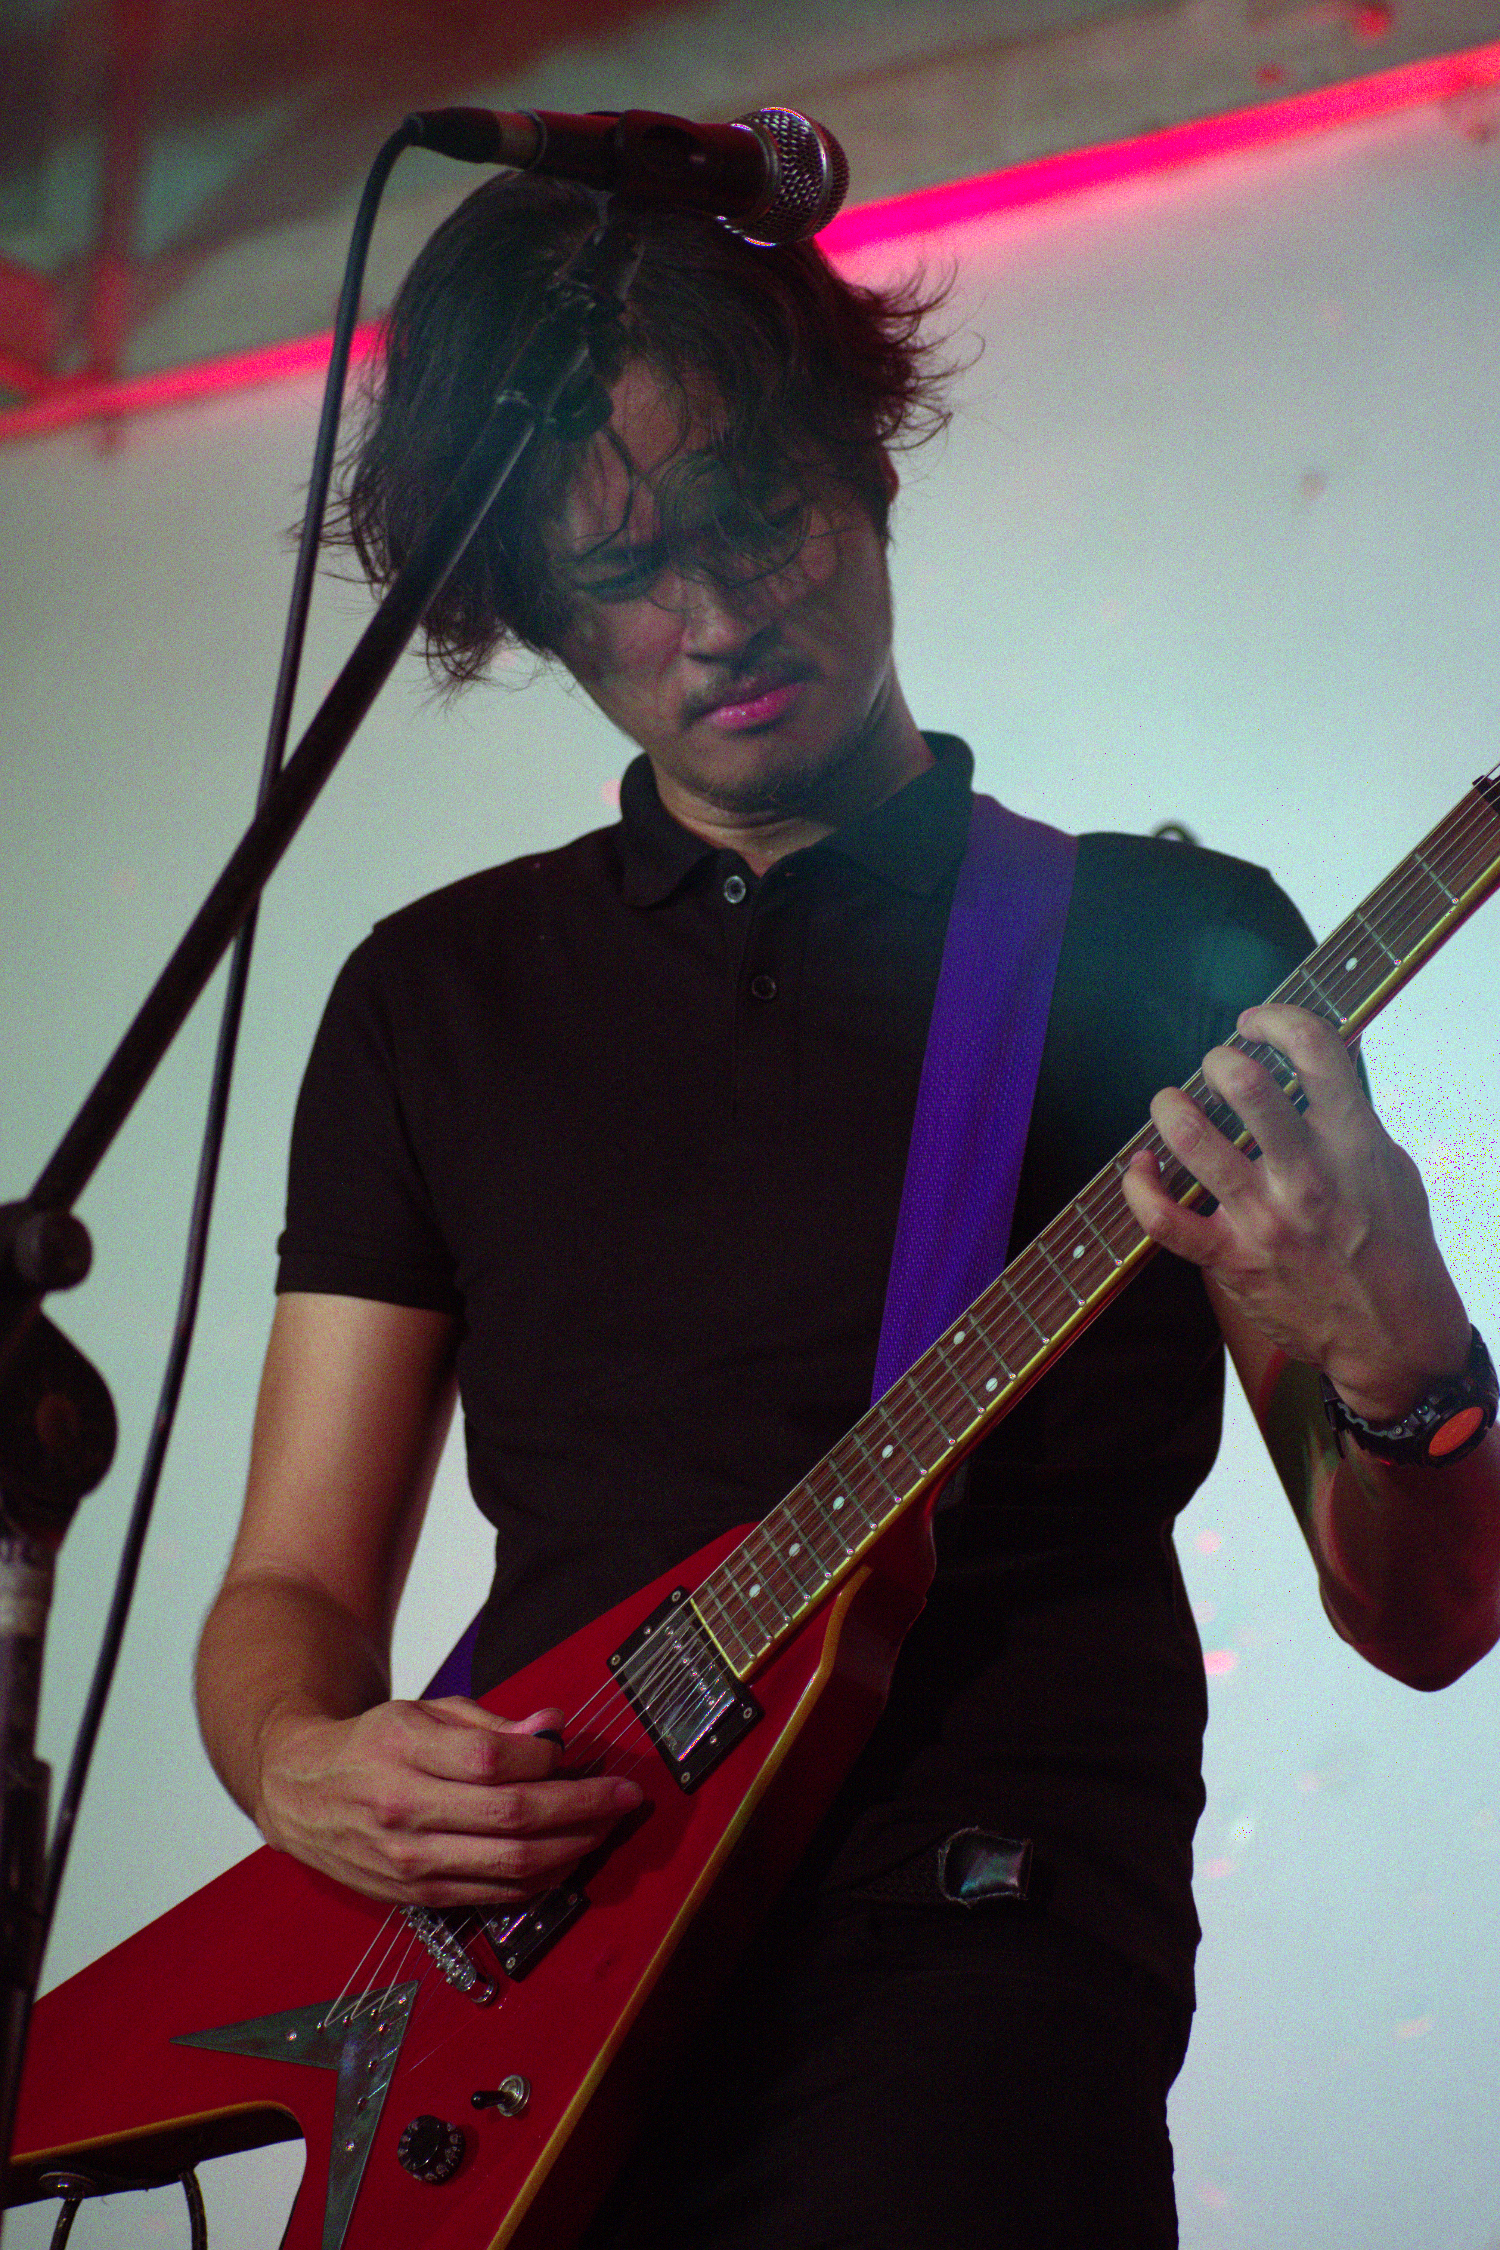
\includegraphics[width=\textwidth]{contrast_stretch.png}
		\caption{Contrast stretched}
		\label{fig:constretch}
	\end{subfigure}
	\begin{subfigure}[h!]{0.24\textwidth}
		\centering
		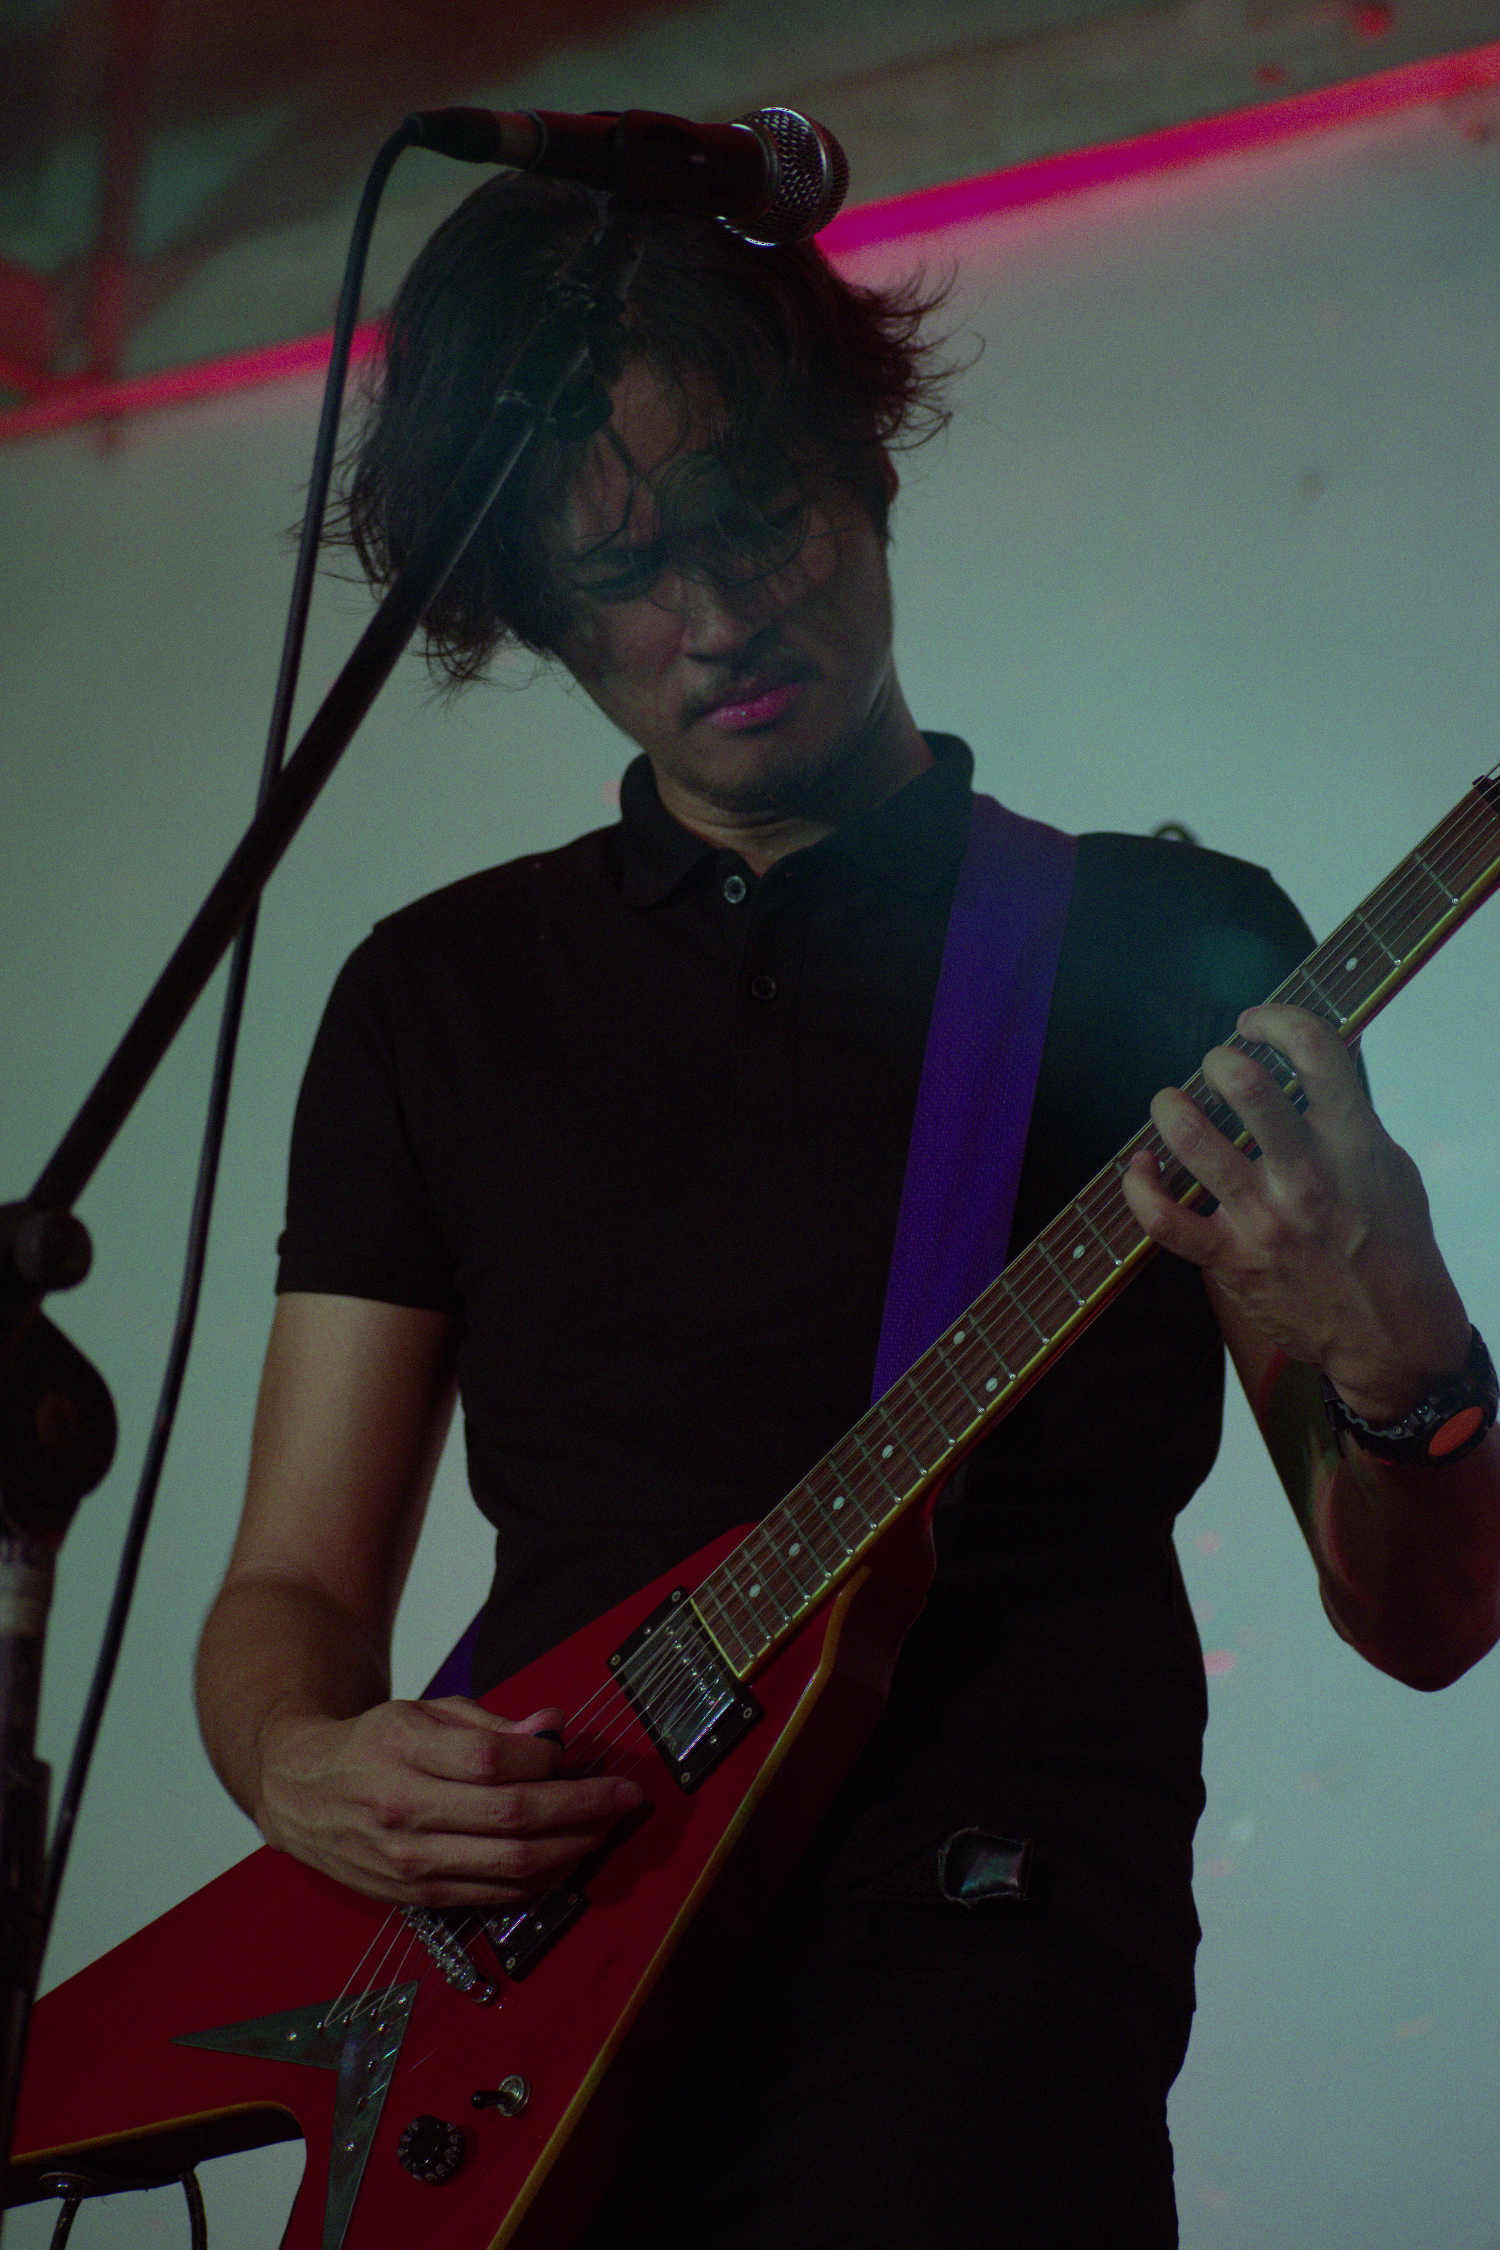
\includegraphics[width=\textwidth]{grayworld.png}
		\caption{Gray world}
		\label{fig:grayworld}
	\end{subfigure}
	\begin{subfigure}[h!]{0.24\textwidth}
		\centering
		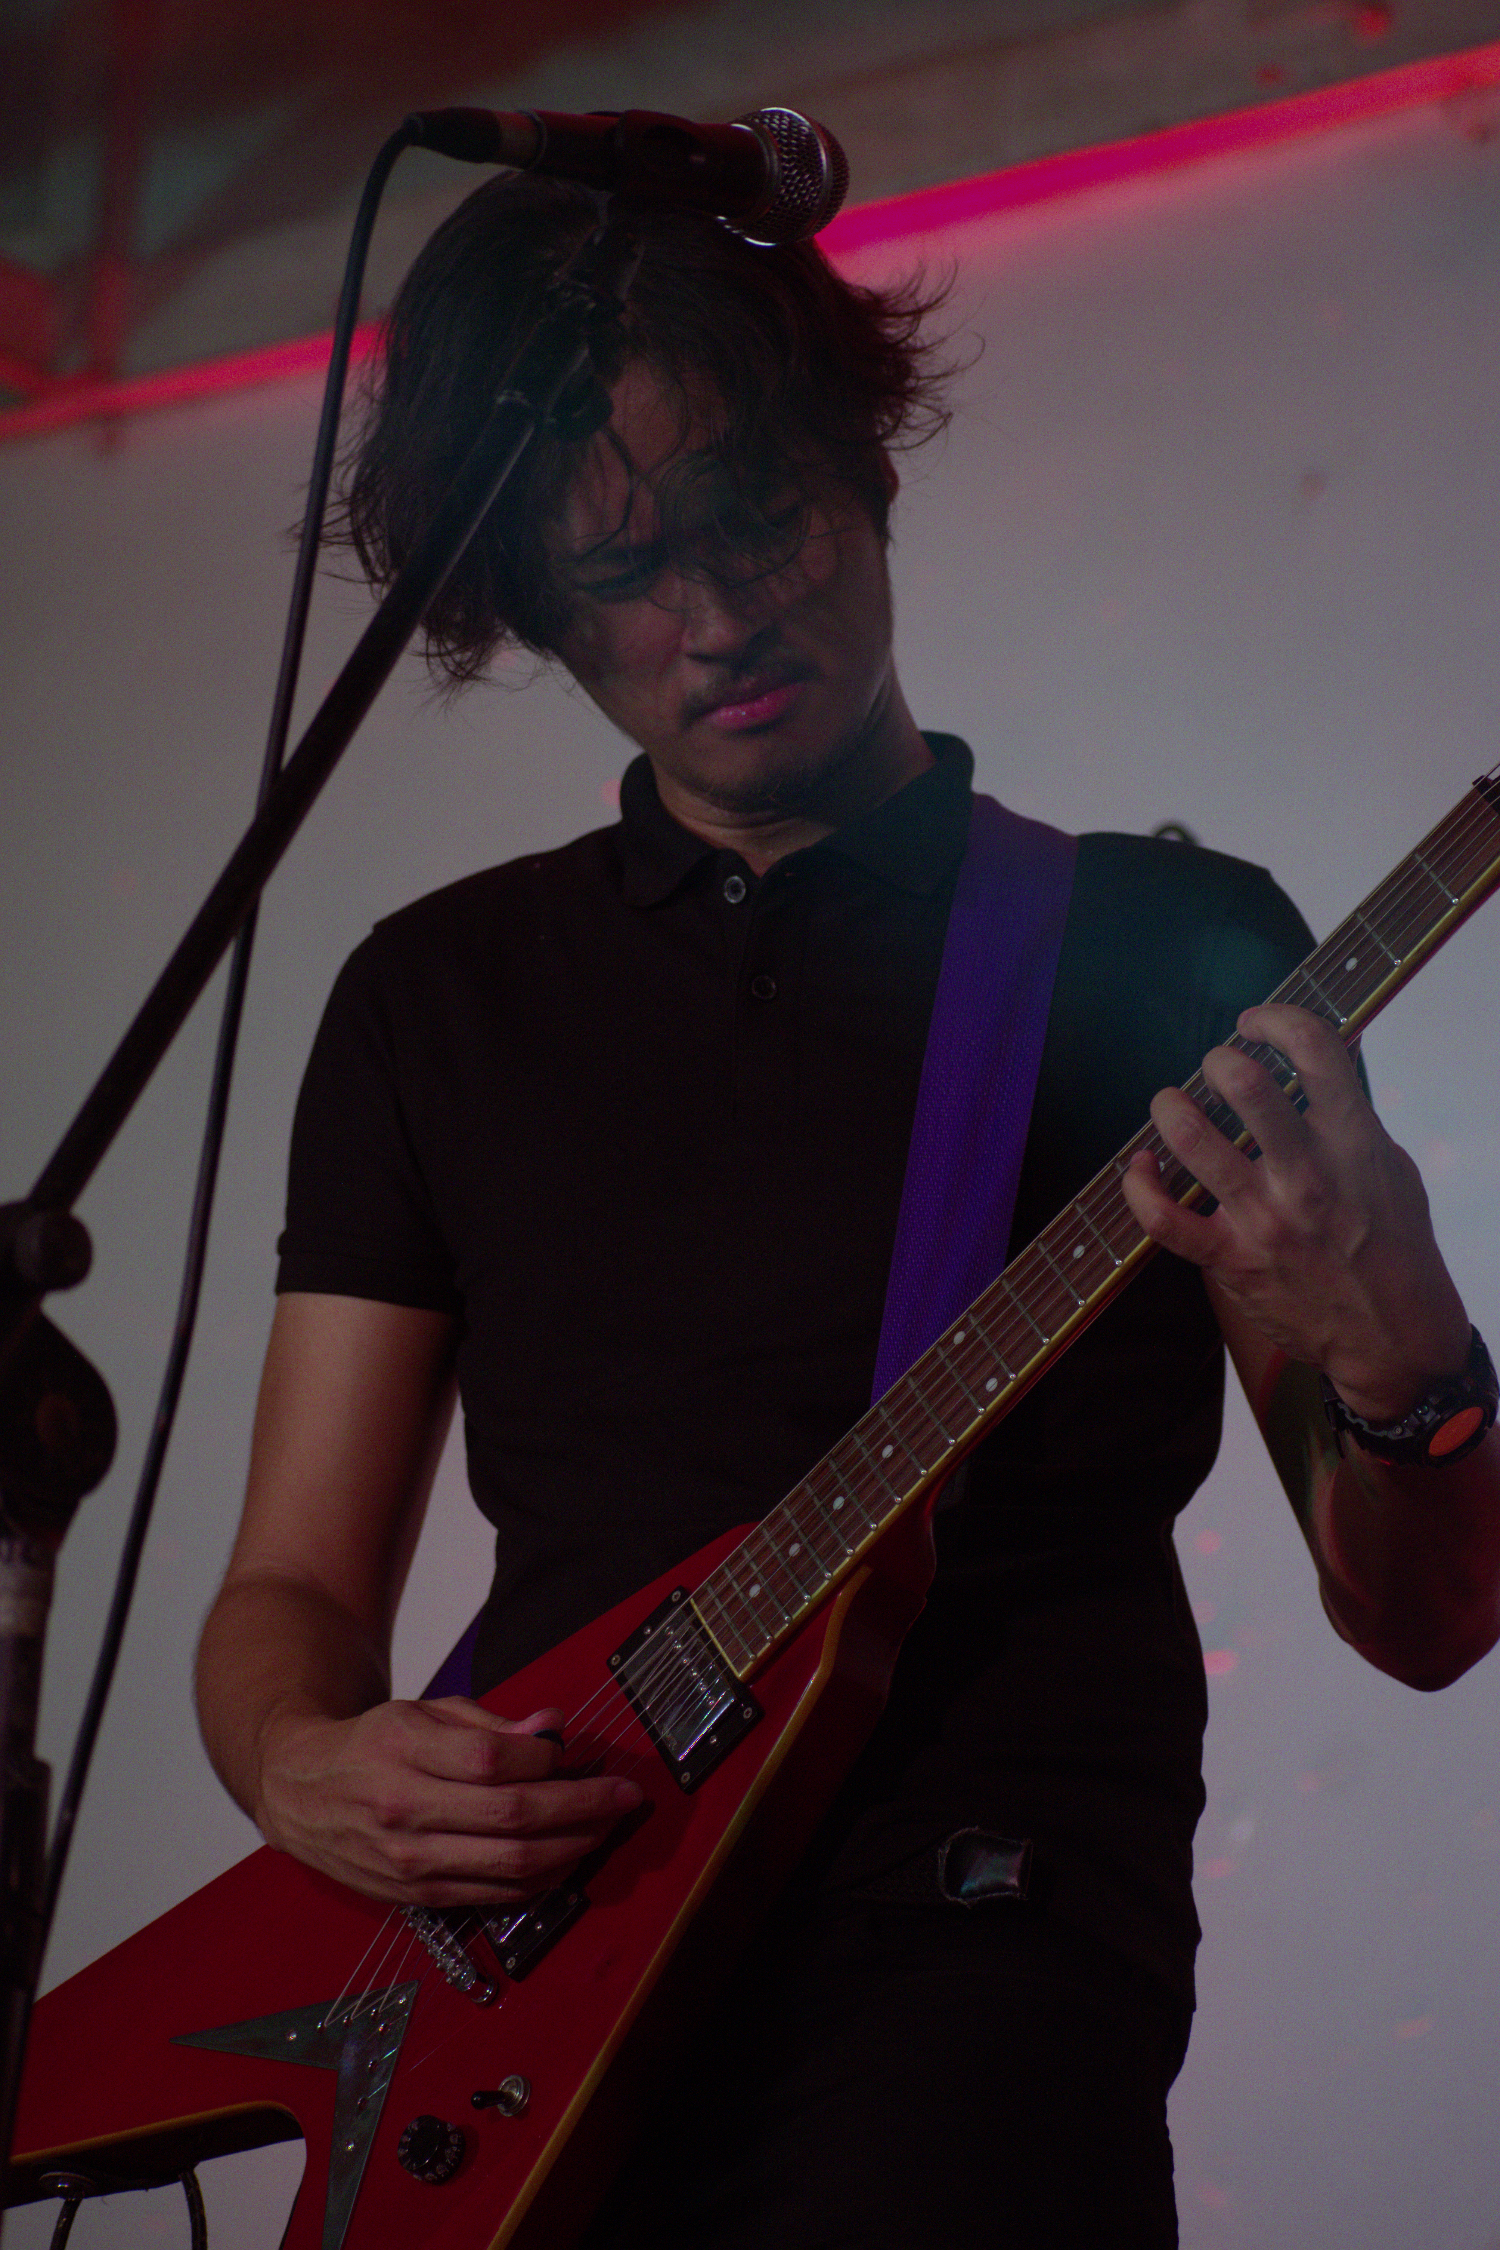
\includegraphics[width=\textwidth]{whitepatch.png}
		\caption{White patch}
		\label{fig:whitepatch}
	\end{subfigure}
	
	\begin{subfigure}[h!]{0.24\textwidth}
		\centering
		\includegraphics[width=\textwidth]{orig_hist.png}
		\caption{}
		\label{fig:orig-hist}
	\end{subfigure}
	\begin{subfigure}[h!]{0.24\textwidth}
		\centering
		\includegraphics[width=\textwidth]{cs_hist.png}
		\caption{}
		\label{fig:cs-hist}
	\end{subfigure}
	\begin{subfigure}[h!]{0.24\textwidth}
		\centering
		\includegraphics[width=\textwidth]{gw_hist.png}
		\caption{}
		\label{fig:gw-hist}
	\end{subfigure}
	\begin{subfigure}[h!]{0.24\textwidth}
		\centering
		\includegraphics[width=\textwidth]{wp_hist.png}
		\caption{}
		\label{fig:wp-hist}
	\end{subfigure}
	
	\caption{Image enhanced using different algorithms (top) and their respective histograms (bottom).}
	\label{fig:manip}
\end{figure}

\begin{figure}[htb]
	\centering
	\includegraphics[width=0.85\textwidth]{patch.png}
	\caption{Extracted white patch location. The size of the bounding box has been exaggerated for easy location. The object of interest is the fret marker on the upper portion of the box.}
	\label{fig:patch}
\end{figure}

\subsection{Auto White Balance Algorithm through Average Equalization and Threshold (AWBAAET)}
To combine everything, \citep{awbaet} proposes a method that modifies the gray world and contrast stretching algorithms and uses a weighted sum of them to perform automatic white balancing. The modified gray world algorithm is as follows:

\begin{equation}\label{eq:gw-mod}
	I_C^\prime = I_C + (\ev{A} - \ev{C})
\end{equation}

and the modified contrast stretching as follows:

\begin{equation}\label{eq:cs-mod}
	I_C^\prime = \frac{I_C - C_{low}}{C_{high} - C_{low}} \times I_{\max} + I_{\min}
\end{equation}

\noindent
where $C_{low}$ and $C_{high}$ are the lower and upper thresholds, respectively, and $I_{\min}$ and $I_{\max}$ are the overall maximum and minimum pixel values, respectively. The image intensity values are scaled according to the thresholds and not the extrema as to avoid over-stretching. The weight is then calculated as follows:

\begin{equation}\label{eq:weights}
	w = \frac{\abs{\ev{C_b} - \ev{C_r}} + \abs{\max{\textrm{std}} - \min{\textrm{std}}}}{n}
\end{equation}

\noindent
where $\ev{C_b}, \ev{C_r}$ are calculated by converting the image to $\mathrm{YC_rC_b}$ color space and taking the averages of the $C$ channels, and std are the standard deviations of the RGB channels. The paper stated that $n$ was a constant taken to be 200 and was obtained experimentally, but do not elaborate on how exactly it was obtained. Essentially, $w$ is the weight of the heavy color cast. The final image is obtained by

\begin{equation}\label{eq:awbaaet}
	I^\prime = w \cdot I_\mathrm{CS} + \qty(1-w) \cdot I_\mathrm{GW}
\end{equation}

\noindent
where $I_\mathrm{CS}$ and $I_\mathrm{GW}$ are the images enhanced using the modified contrast stretching and gray world algorithms, respectively. The result is shown in Fig. \ref{fig:awbaaet} alongside the other algorithms for comparison. Because of the heavy red color cast in the original image, the CS portion of the algorithm is given a greater weight, so the final image looks more like the CS-corrected image.

\begin{figure}[htb]
	\centering
	\begin{subfigure}[h!]{0.3\textwidth}
		\centering
		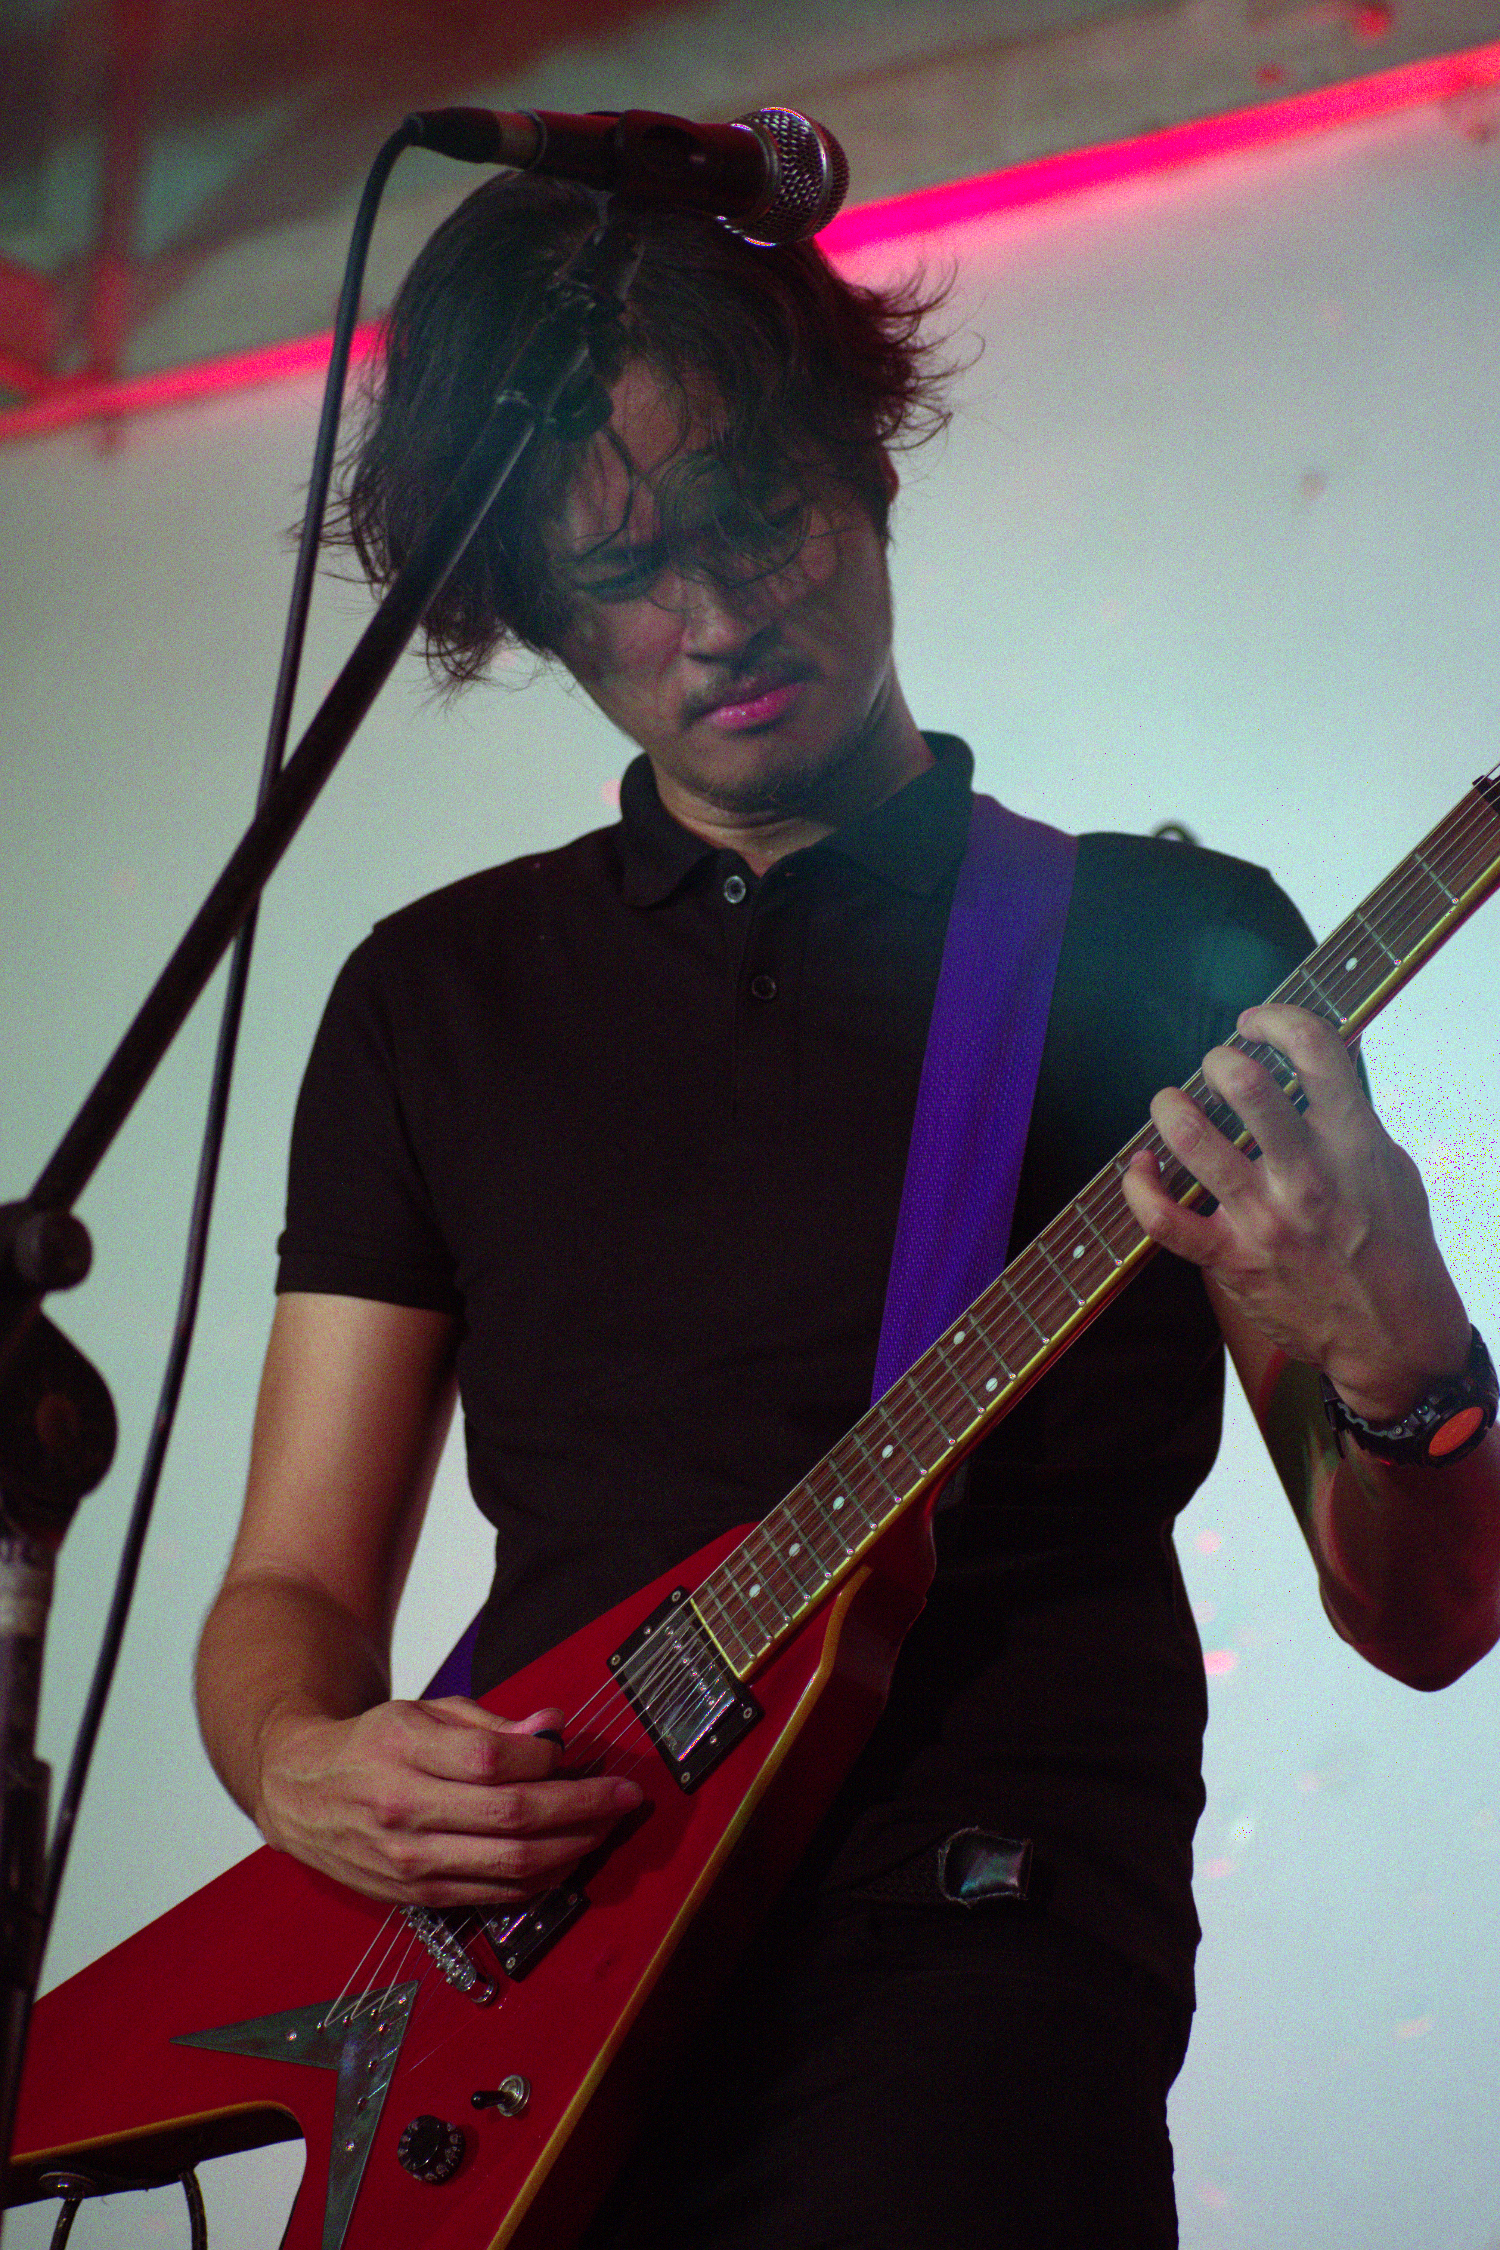
\includegraphics[width=\textwidth]{contrast_stretch.png}
		\caption{CS}
		\label{fig:constretch-com}
	\end{subfigure}
	\begin{subfigure}[h!]{0.3\textwidth}
		\centering
		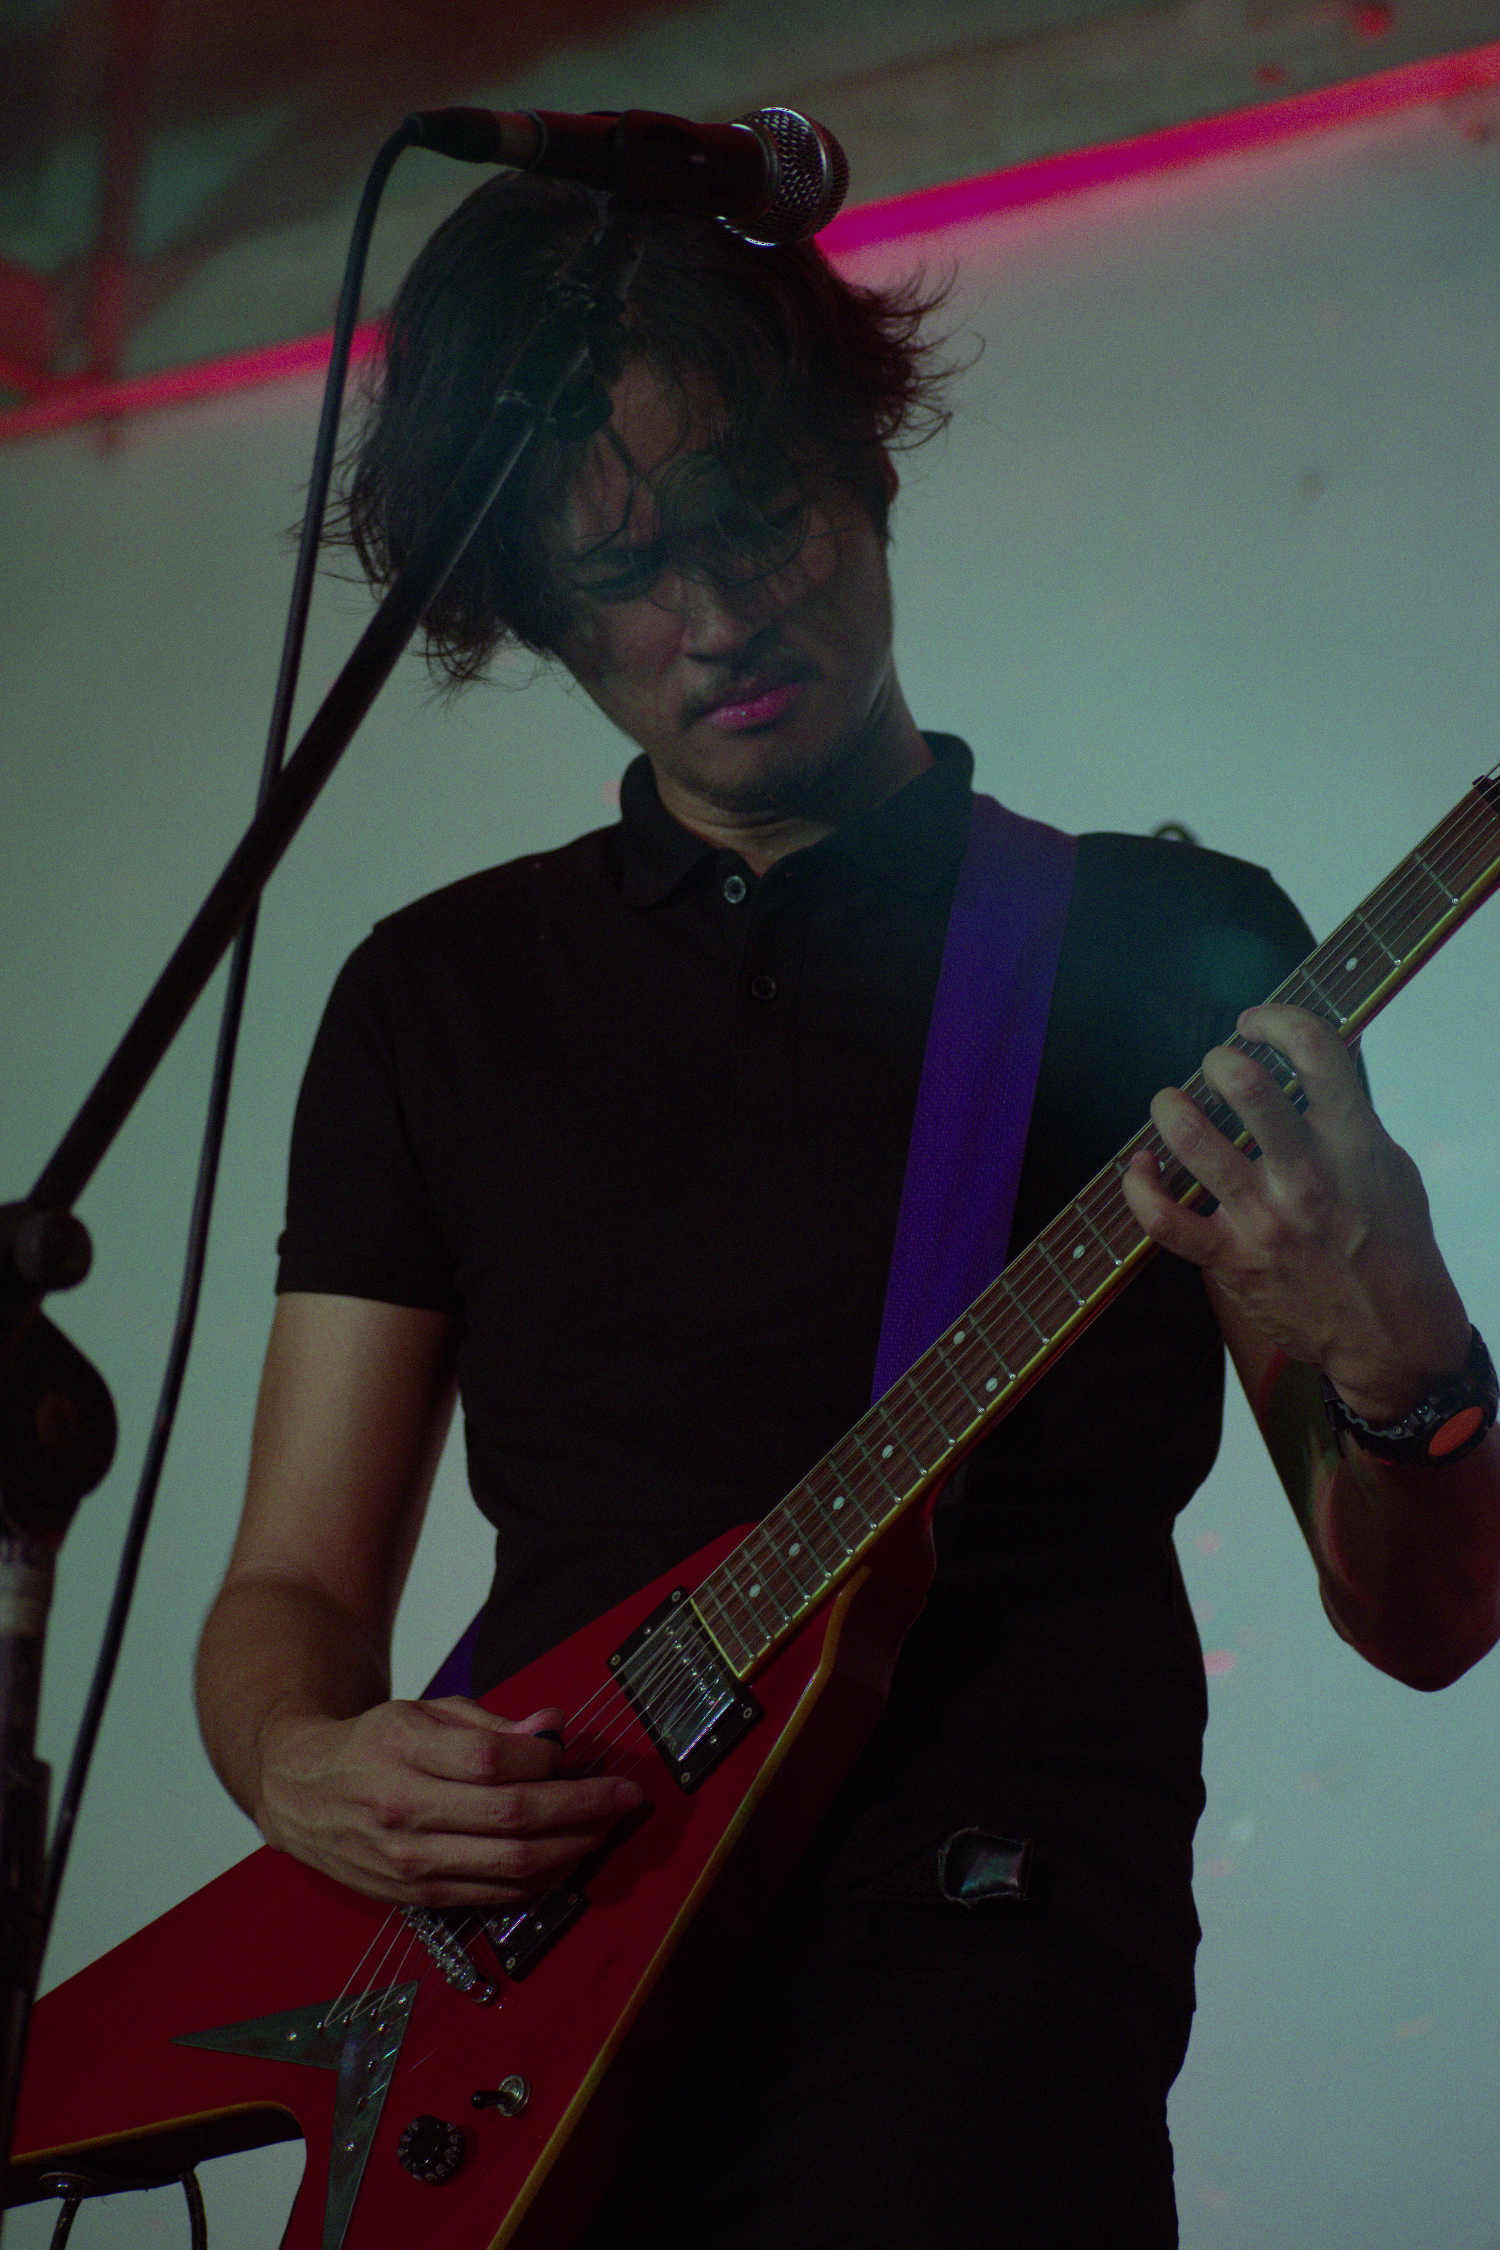
\includegraphics[width=\textwidth]{grayworld.png}
		\caption{GW}
		\label{fig:grayworld-com}
	\end{subfigure}
		\begin{subfigure}[h!]{0.3\textwidth}
		\centering
		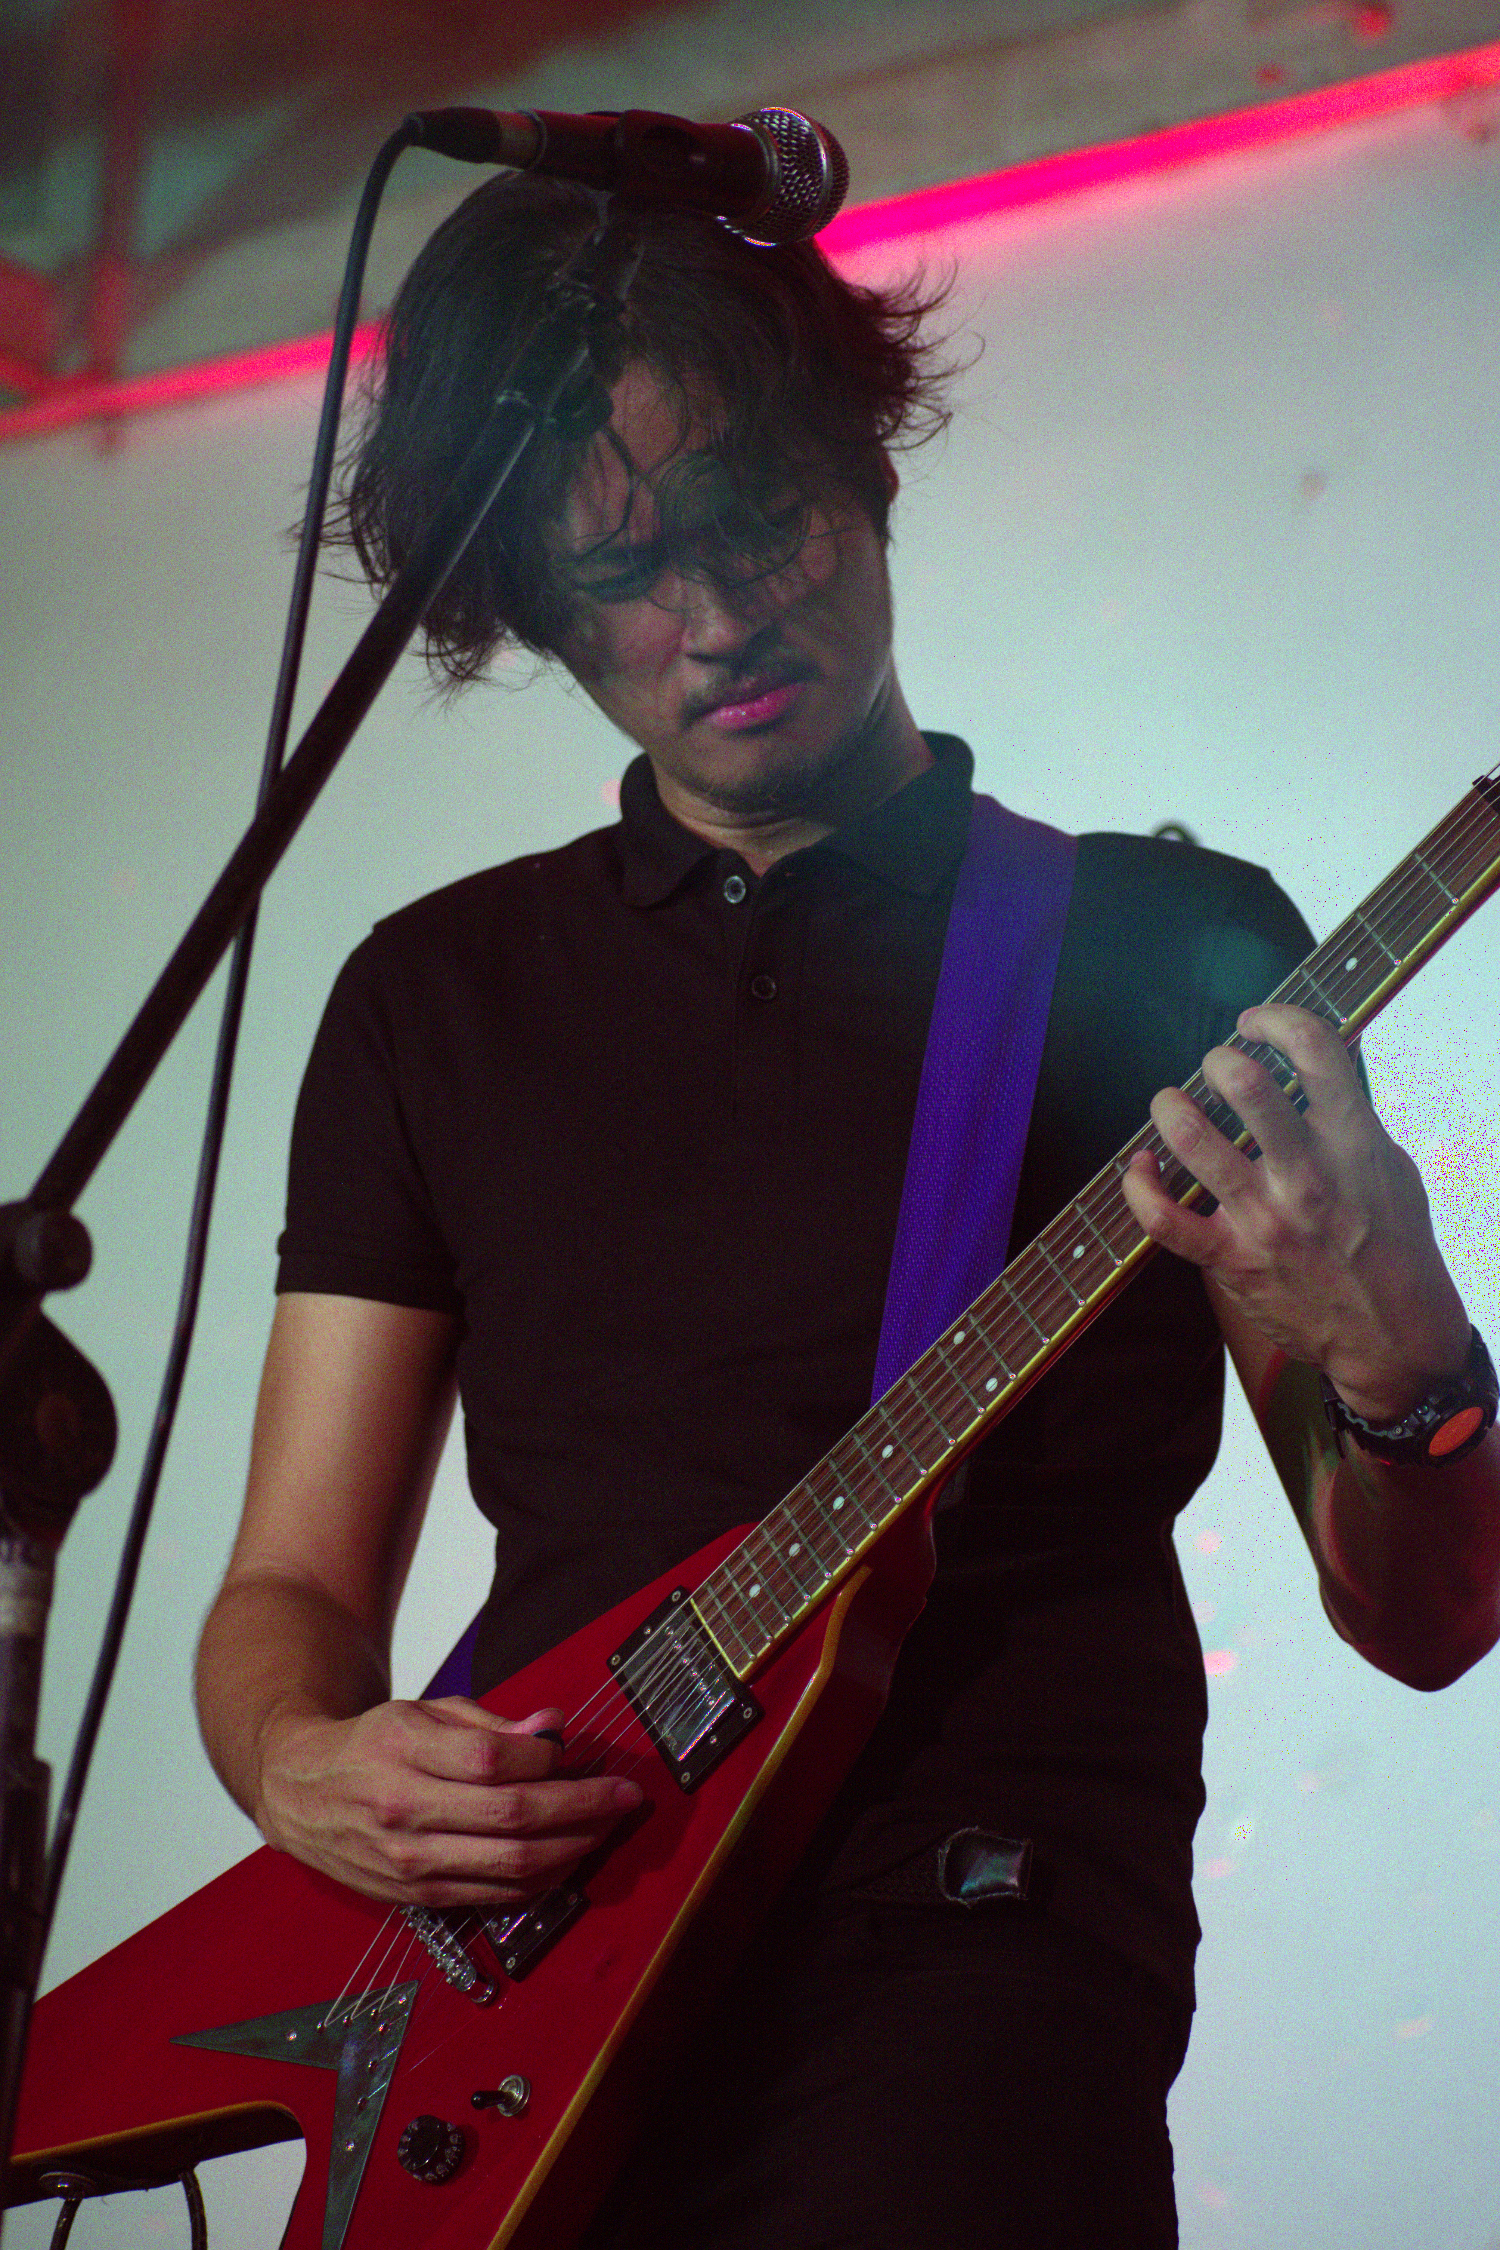
\includegraphics[width=\textwidth]{awbaaet_out.png}
		\caption{AWBAAET}
		\label{fig:awbaaet}
	\end{subfigure}
	
	\begin{subfigure}[h!]{0.3\textwidth}
		\centering
		\includegraphics[width=\textwidth]{cs_hist.png}
		\caption{}
		\label{fig:cs-hist-com}
	\end{subfigure}
	\begin{subfigure}[h!]{0.3\textwidth}
		\centering
		\includegraphics[width=\textwidth]{gw_hist.png}
		\caption{}
		\label{fig:gw-hist-com}
	\end{subfigure}
		\begin{subfigure}[h!]{0.3\textwidth}
		\centering
		\includegraphics[width=\textwidth]{awbaaet_hist.png}
		\caption{}
		\label{fig:awbaaet-hist}
	\end{subfigure}
	
	\caption{Comparison of the different auto white balance algorithms.}
	\label{fig:comparisons}
\end{figure}

\begin{table}[!htb]
	\centering
	\caption{Self-evaluation.}
	\begin{tabular}{|r|c|}
		\hline
		Technical correctness & 5 \\ \hline
		Quality of presentation & 5 \\ \hline
		Initiative & 2 \\ \hline
		\textbf{TOTAL} & \textbf{12} \\ \hline
	\end{tabular}
	\label{tab:self-eval}
\end{table}

\bibliographystyle{spp-bst}
\bibliography{186-Act6}

\end{document}